\documentclass{article}
\usepackage[utf8]{inputenc}

\title{TCP/IP communication flows into sentence-like transcriptions}
\author{Allan Kálnay}
\date{\today}

\usepackage{natbib}
\usepackage{graphicx}
\usepackage{hyperref}


\begin{document}
\sloppy

\maketitle

\section*{Abstract}
The goal of this work was to design a suitable schema that transforms TCP/IP flows into sentence-like transcriptions and implement a software in Python that does such transformation from \textit{pcap} files and to evaluate its suitability for attack detection.

The schema that we implemented uses printable ASCII characters in the range from the exclamation mark character (\textit{!}) up to the tilde character (\textit{$\sim$}) which makes 93 characters altogether. Our schema utilizes three network flow features to express the final transcription -- packet length, flow direction and inter packet times. With a specific configuration that we used for these four features, we were able to to convert huge pcap files (approximately 10GB) into few kB big files containing the sentence-like transcriptions of the network flows contained in those pcap files.

At the same time we were able to produce quite decent results for a binary classification problem distinguishing between attack and non-attack flows. For this purpose we used Random Forest Classifier on top of a basic bag of words data set constructed from the sentence-like transcriptions.

\newpage
\tableofcontents
\newpage

\section{Background}
\subsection{pcap2transcription}
pcap2transcription \cite{pcap2transcription} is a preliminary project that tries to solve the same problem as our project tries. The project uses a similar technique for creating the transcription schema. It deals with IP packet lengths and flow directions the same as our project does. Uppercase symbols describe a communication in one direction and the lower case symbols describe the communication in the other direction. The dash character (\textit{-}) stands for 10ms without packet exchange (communication gap/silence). Also, the project does not work efficiently when it comes to feature extraction as well as memory. We improved these two in our project. The pcap2transcription project is basically a base for our project.


\section{Methodology}
\subsection{Data}\label{sec-data-cic-ids-2017}
For the purpose of our experiments we used the synthetic CIC IDS 2017 data set \cite{sharafaldin2018toward}. The data set contains pcap files and labels of the network flows. The labels are binary -- attack and non-attack.

There are 5 different pcap files in this data set. Each of them represents a different day in the week from Monday to Friday. The size of all of them vary from 7GB up to 14GB.

Table \ref{tab:cic-ids2017-data-description} describes the data sets contained in the CIC IDS 2017 data in terms of network flows, attacks and non-attacks

\begin{table}[h!]
\centering
    \begin{tabular}{ |c|c|c|c| }
        \hline
        Day & \# network flows & \# non-attacks & \# attacks \\
        \hline
        Monday & $96\ 784$ & $96\ 784$ & 0 \\
        Tuesday & $80\ 898$ & $80\ 887$ & $11$ \\
        Wednesday & $80\ 716$ & $80\ 662$ & $54$ \\
        Thursday & $77\ 069$ & $75\ 948$ & $1\ 121$ \\
        Friday & $73\ 726$ & $73\ 534$ & $192$ \\
        \hline
    \end{tabular}
\caption{CIC IDS 2017 data description table}
\label{tab:cic-ids2017-data-description}
\end{table}


\noindent\textbf{Labeling}

The official page of CIC IDS 2017 data\footnote{\url{https://www.unb.ca/cic/datasets/ids-2017.html}} guides you on how to do the data labeling of all days contained in the data set. However, we were provided with a labeling script by Félix Iglesias Vázquez and Fares Meghdouri which we highly appreciate. We double-checked the rules for labeling in the script and approved it for our use.


% describe how many packets do the files contain

%-------------------------------------------------------
\subsection{Data Exploration}\label{sec-dataset-exploration}
% describe what I found in data -- show the charts from the 1st and 2nd report for Felix, describe these findings and later
Since the beginning we decided to work with several network flow features -- protocol identifier, packet length, communication gaps (communication silence), communication direction, packet timestamp. Based on this decision we researched our data set to find out more about these features and to drive our decisions later based on our findings.

The protocol identifier was purely used for identification whether a packet is a TCP/IP packet or not. If it is not a TCP/IP packet, then, as the name of the project suggests, we do not care about the packet. If it is a TCP/IP packet, we work with that.

\subsubsection{Packet Size}
As \cite{oreilly-tcp} states, the minimum size of a TCP/IP packet is 21 bytes and the maximum size of such packet is $65\ 535$ bytes. We analysed the cumulative distribution function (CDF) of packet sizes of the packets of all CIC-IDS 2017 days. The output of our analysis is the figure \ref{fig-cdf-packet-sizes}. The figure provides us with information of what percentage of packets have size less than or equal to a certain value. The figure shows that almost all of the packets of all days are less than or equal to 5kB.

\begin{figure}[tbp!]
  \centering
  \begin{minipage}[b]{0.49\textwidth}
    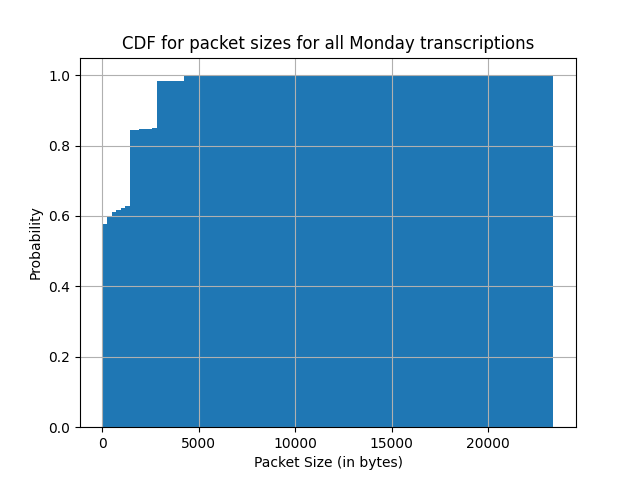
\includegraphics[width=\textwidth]{final-report/img/data-analysis/ipTotalLength_cdf/Monday_packet-sizes_cdf.png}
  \end{minipage}
  \hfill
  \begin{minipage}[b]{0.49\textwidth}
    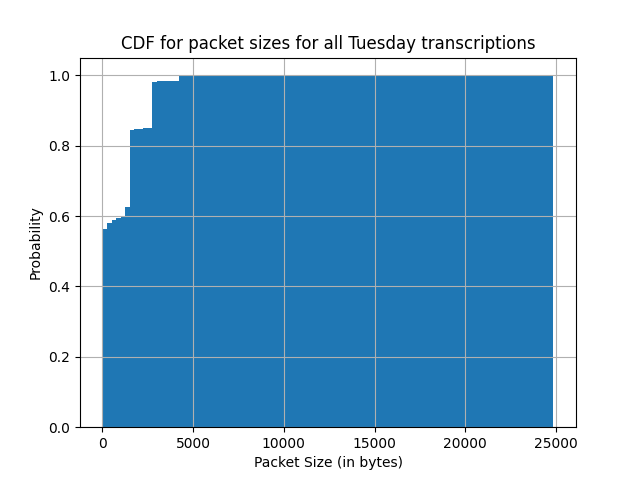
\includegraphics[width=\textwidth]{final-report/img/data-analysis/ipTotalLength_cdf/Tuesday_packet-sizes_cdf.png}
  \end{minipage}
  \vfill
  \begin{minipage}[b]{0.49\textwidth}
    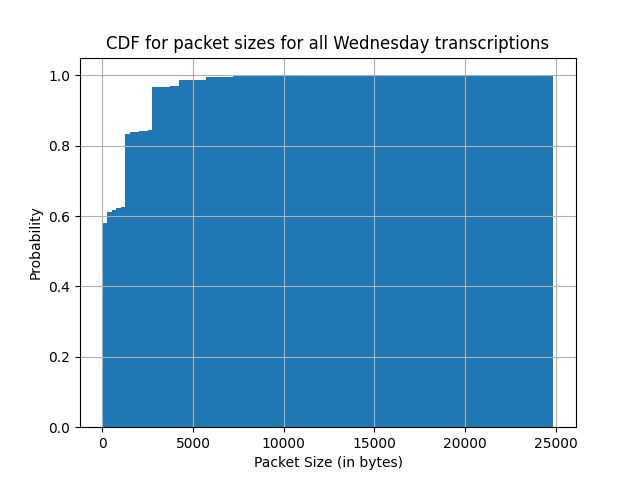
\includegraphics[width=\textwidth]{final-report/img/data-analysis/ipTotalLength_cdf/Wednesday_packet-sizes_cdf.png}
  \end{minipage}
  \hfill
  \begin{minipage}[b]{0.49\textwidth}
    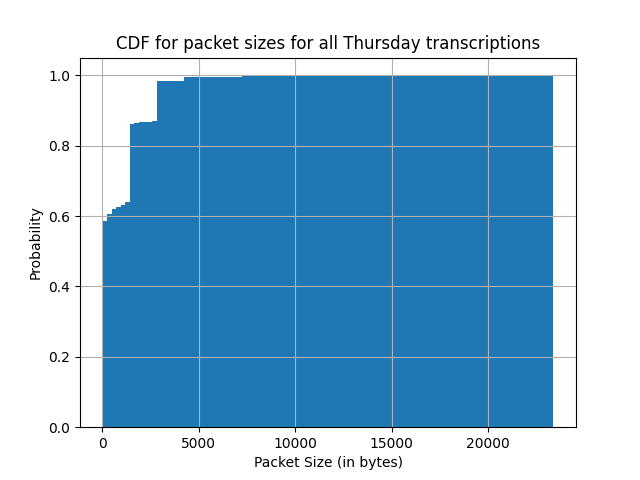
\includegraphics[width=\textwidth]{final-report/img/data-analysis/ipTotalLength_cdf/Thursday_packet-sizes_cdf.png}
  \end{minipage}

  \vfill

  \begin{minipage}[b]{0.49\textwidth}
    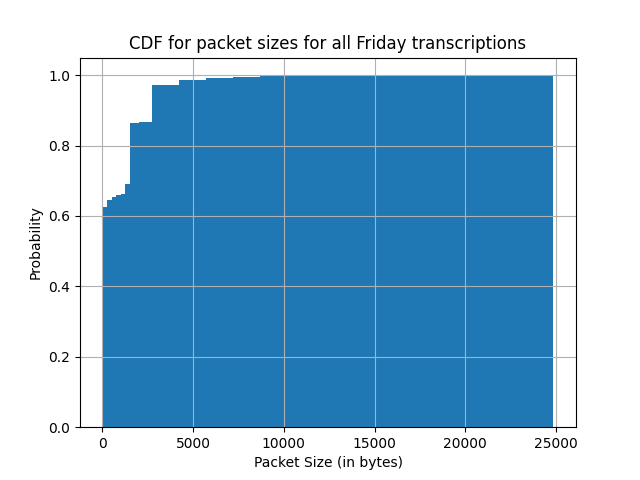
\includegraphics[width=\textwidth]{final-report/img/data-analysis/ipTotalLength_cdf/Friday_packet-sizes_cdf.png}
  \end{minipage}

  \caption{CDF plots for packet sizes of all CIC-IDS 2017 days}
  \label{fig-cdf-packet-sizes}
\end{figure}
%-------------------------------------------------------



%-------------------------------------------------------
\subsection{Transcription Schema Description}\label{sec-schema}

\subsubsection{Feature extraction}

Our transcription schema utilizes several network flow features. Among these are also the features that determine how output transcription schema will look like. These are:

\begin{itemize}
    \item \textit{packet length},
    \item \textit{flow direction},
    \item \textit{inter packet time}.
\end{itemize}

These three are basic features that can be easily extracted from both encrypted and non-encrypted network communication. Moreover, the results from the research \cite{meghdouri2018analysis} show that packet length based features are a decisive factor for identifying malicious activity.


% The first two are used because they are obvious and can easily help us with providing more information about the flows. The 3rd one is used for multiple purposes. The second reason is that we decide the communication silences based on the time differences of two consecutive packets.

% The output of our data processing pipeline is a tsv file with four columns -- Source IP, Destination IP, Attack, Transcription. The IP addresses represent the communication endpoints. The Attack attribute contains a binary information whether the network flow is an attack or not. The Transcription attribute contains the transcription itself.

\subsubsection{Transcriptions}\label{sec-transcriptions}

A transcription is a string of characters describing a network flow. We use 93 characters for constructing a transcription string. These are printable ASCII characters in the range from the exclamation mark character (\textit{!}) up to the tilde character (\textit{$\sim$}) where each character represents a captured packet length. Each character represents different packet lengths. Transcription string characters are ordered in the same chronological order as the packet captures.

The very first character, exclamation mark, is used to represent a silence in a communication. One exclamation mark represents a silence of 1 second. The 46 characters starting from the quotation mark included up to the \textit{O} character included are used to describe one direction of a communication. The 46 characters starting from the \textit{P} character included up to the tilde character included are used to describe the other direction of a communication. The meaning of transcription characters is captured in a tabular form in the table \ref{tab:character-meanings}.

\begin{table}[h!]
\centering
\begin{tabular}{ |p{0.35\linewidth} | p{0.6\linewidth}| }
 \hline
 Character & Meaning \\
 \hline \hline
 ! & Silence in a communication of 1s time period. \\
 \hline
 " up to O & A packet sent from host A to host B. Each of these characters represents different packet length bucket. \\
 \hline
 P up to $\sim$ & A packet sent from host B to host A. Each of these characters represents different packet length bucket. \\
 \hline
\end{tabular}
\caption{Meaning of transcription characters}
\label{tab:character-meanings}
\end{table}

Based on the research in the section \ref{sec-dataset-exploration} we utilized the characters in such way that the characters represent different bins of packet lengths. We reasonably chose binning based on the analysis of the figure \ref{fig-cdf-packet-sizes}. We encoded the packets of lengths $<= 2^{14}$ with first 30 characters, the packets of lengths $(2^{14}; 2^{16}]$ with the next 15 characters and the packets of lengths $> 2^{16}$ with the last (46th) character. Naturally, each communication direction utilizes its own character set as described in the section \ref{sec-dataset-exploration}. In every category the bins are of the same size. Meaning, in the first category there are 30 bins of the same size, in the second category there are 15 bins of the same size and in the last category there is just one bin.

\noindent An example transcription may look like this:

$$ CCn!D!n $$

\noindent The meaning of the transcription character by character is the following:

\begin{enumerate}
    \item C -- host A sent a packet of length between 8752B up to 9298B
    \item C -- host A sent a packet of length between 8752B up to 9298B
    \item n -- host B sent a packet of length between 15863B up to 16384B
    \item ! -- 1s of communication silence
    \item D -- host A sent a packet of length between 9299B up to 9846B
    \item ! -- 1s of communication silence
    \item n -- host B sent a packet of length between 15863B up to 16384B
\end{enumerate}

%-------------------------------------------------------



%-------------------------------------------------------


\subsection{Implementation}
% describe the software itself, the scripts for data processing, what language I used

\subsubsection{Data Processing Pipeline}
The software for processing the \textit{pcap} files and converting network flows into sentence-like transcriptions is a data processing pipeline consisted of two steps. The two-step process consists of extracting the necessary features from a \textit{pcap} file with \textit{go-flows} software \cite{goflows-reference} and the 2nd step is the transcriptions building process itself based on the output from the 1st step. The data processing pipeline itself is a shell script that orchestrates the steps to be done in order to achieve the final output. The path to the script is \verb|experiments/01/transcription/pipeline-general.sh|


\subsubsection{go-flows Features Extraction}\label{sec:go-flows-feature-extraction}
First step of data processing pipeline is extracting features from a pcap file using go-flows. go-flows uses a configuration file which describes what features we want to extract from a pcap. The configuration file for go-flows used in our data processing pipeline is located in \verb|/transcription/feature_extraction/2tuple_bidi.json|. This configuration file makes go-flows produce a CSV file containing network flows with following features:

\begin{itemize}
    \item \textit{flowStartMilliseconds} -- beginning of a flow timestamp in ms,
    \item \textit{flowDurationMilliseconds} -- flow duration in ms,
    \item \textit{sourceIPAddress} -- source IP address of a flow,
    \item \textit{destinationIPAddress} -- destination IP address of a flow,
    \item \textit{accumulate(ipTotalLength)} -- accumulated lengths of packets -- array,
    \item \textit{accumulate(\textunderscore interPacketTimeMilliseconds)} -- accumulated inter packet times in ms -- array,
    \item \textit{accumulate(flowDirection)} -- accumulated flow directions related to packets -- array.
\end{itemize}
Each row of the output CSV file represents a single network flow.


\subsubsection{Transcriptions Maker}
As mentioned above, the 2nd step of the data processing pipeline is the transcriptions building process. This is the core software of this project implemented in Python expecting a CSV file of a certain structure as an input and producing a TSV file containing the sentence-like transcriptions as the output among other features described in the section \ref{sec-output-dataset}. Let's call this software the transcription maker.

The input CSV file for this core software is an output produced from go-flows. All the necessities for this input CSV file are described in the section \ref{sec:go-flows-feature-extraction}.

Transcription maker read the input CSV file line by line (a.k.a. flow by flow) and traverse the array features in order to produce the output characters building the final transcription strings.

The final structure of the output TSV file produced by the transcription maker software is described in the section \ref{sec-output-dataset}.

The source code of the transcriptions maker software is located in the project's repository in the path \verb|/experiments/01/transcription/src/main/python/transcription|.

%---------------------------------------------------------------------

\subsubsection{Output Data Set}\label{sec-output-dataset}

The output data set containing transcriptions derived from pcap files is a TSV file. The output file contains 5 columns. These are:
\begin{itemize}
    \item \textit{flowStartMilliseconds} -- flow start in milliseconds,
    \item \textit{flowDurationMilliseconds} - flow duration in milliseconds,
    \item \textit{sourceIPAddress} -- source IP address of a flow,
    \item \textit{destinationIPAddress} -- destination IP address of a flow,
    \item \textit{transcription} -- the transcription string itself.
\end{itemize}
%---------------------------------------------------------------------

\section{Evaluation}

\subsection{CIC-IDS2017 Data Set Experiments}\label{sec-cic-ids-experiments}

The experiments provided in this section were conducted on top of the CIC-IDS2017 data set described in the section \ref{sec-data-cic-ids-2017}. As the whole data set consists of several sub data sets, we conducted experiments on top of almost each one of these sub data sets.

As Monday data do not have any malicious traffic, we skipped this one. All the data sets from Tuesday to Friday contain both malicious and non-malicious traffic, therefore we conducted an experiment on top of each of them.

From each data set from Tuesday to Friday, we derive two different data sets for training and evaluating two different models. Both of these models are trained for binary classification, meaning deciding between the two classes -- \textit{attack} and \textit{non-attack}.

For both the baseline and non-baseline models we split both attacks and non-attacks in the 70:30 train set to test set ratio. Then we merge non-attacks with attacks for both train and test data separately in order to create a single train set and a single test set.

We didn't necessarily train and test our baseline models on exactly the same train and test network flows as we did for the models on top of transcriptions data. Nevertheless, we subsampled from the same sets of network flows which minimizes the impact of not using the same network flows for training and testing the models. The counts for train and test sets are exactly the same for both models in each day, i.e. if Thursday's baseline model has a train set consisted of $1\ 500$ non-attacks and $100$ attacks and a test set consisted of $700$ non-attacks and $50$ attacks, then the same counts for train and test sets are applied to the Random Forest on top of bag of words model.

The goal for these experiments was to achieve the highest possible accuracy for both the \textit{attack} class and the \textit{non-attack} class. Achieving overall accuracy on top of whole test sets is meaningless for us as our data sets are imbalanced and therefore overall accuracy may distort results.\\


\noindent\textbf{Baseline Model}

As a baseline model we chose to train Random Forest models. We aggregated several network flow features in order to create data sets of numeric vectors. We used the very same network flow features for constructing these numeric vectors of the data sets as the ones that we use for constructing transcriptions. These features are:

\begin{itemize}
    \item \textit{packet length},
    \item \textit{flow direction},
    \item \textit{inter packet time}.
\end{itemize}

\noindent For each \textit{flow direction} (forward/backward) we used each of these aggregation functions on top of the \textit{packet length} and \textit{inter packet time} features:

\begin{itemize}
    \item \textit{min},
    \item \textit{max},
    \item \textit{median},
    \item \textit{mean},
    \item \textit{mode},
    \item \textit{stdev}.
\end{itemize}

\vspace{0.5cm}


\noindent\textbf{Obtained Model}

In the each experiment, we decided to train a Random Forest models on top of bag of words for the transcription data sets comparing them to baseline Random Forest models. We will call the non-baseline models \textit{``obtained models"}.

In the experiments we work with the same schema of transcription data sets as described in the section \ref{sec-output-dataset} and the same transcriptions schema as described in the section \ref{sec-transcriptions}.

We used a bag of words technique to express our transcription strings as numeric vectors. For each entry of the data set (a transcription) we counted number of each word (symbol) in the transcription. Basically, we transformed our data set of transcriptions to the data set where our dimensions represented the word counts in transcriptions. For better understanding, see an example at figure \ref{fig-bag-of-words-example}.

\begin{figure}[h!]
\centering
\begin{tabular}{ |c|c|c|c| }
 \hline
 srcIP & dstIP & attack & transcription \\
 \hline
 1.1.1.1 & 2.2.2.2 & 1 & AAp!D!p \\
 2.2.2.2 & 3.3.3.3 & 0 & P!PD \\
 \hline
\end{tabular}

\vspace{0.3cm}

\begin{tabular}{ |c|c|c|c|c|c|c| }
 \hline
 srcIP & dstIP & A & D & P & p & ! \\
 \hline
 1.1.1.1 & 2.2.2.2 & 2 & 1 & 0 & 2 & 1 \\
 2.2.2.2 & 3.3.3.3 & 0 & 1 & 2 & 0 & 1 \\
 \hline
\end{tabular}
\caption{Data set of transcriptions (top table) and bag of words data set (bottom table)}
\label{fig-bag-of-words-example}
\end{figure}


\clearpage

\subsubsection{Friday}

For this experiment we used the Friday's CIC-IDS 2017 data. We sampled $5\ 500$ non-attacks and used all attacks from this data set. This makes altogether a data set of $5\ 692$ entries.

The predictions of a obtained model gives us very promising results as we can see at Figure \ref{fig-exp1-obtained-model}. The precision scores for both non-attacks and attacks classification are almost the same -- around $92\%$.

The baseline model achieves better results here in regards to predicting non-attacks with $100\%$ precision compared to the obtained model scoring $92.4\%$ precision than the obtained model. In regards to attacks, the models perform exactly same well. The results of the baseline model are captured in the Figure \ref{fig-exp1-baseline}.

\begin{figure}[h!]
    \centering
    \includegraphics[width=0.7\textwidth]{final-report/img/friday/confusion-matrix-normalized.png}

    \centering
    \begin{tabular}{ |c|c|c|c|c|c|c| }
     \hline
      & true non-attack & true attack \\
     \hline
     predicted non-attack & 1525 & 125 \\
     \hline
     predicted attack & 5 & 53 \\
     \hline
    \end{tabular}

    \caption{Confusion matrices with normalized and absolute values of the obtained model for the experiment 1}
    \label{fig-exp1-obtained-model}
\end{figure}



\begin{figure}[h!]
    \centering
    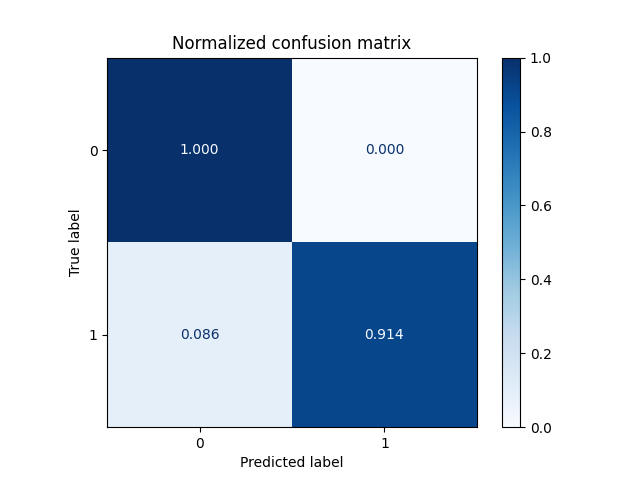
\includegraphics[width=0.7\textwidth]{final-report/img/friday/friday-baseline-normalized.png}

    \centering
    \begin{tabular}{ |c|c|c|c|c|c|c| }
     \hline
      & true non-attack & true attack \\
     \hline
     predicted non-attack & 1635 & 15 \\
     \hline
     predicted attack & 12 & 46 \\
     \hline
    \end{tabular}
    \caption{Confusion matrices with normalized and absolute values of the baseline model for the experiment 1}
    \label{fig-exp1-baseline}
\end{figure}

\clearpage

% describe the results that I got (the confusion matrix, accuracy etc). Next describe how I constructed the train and test data set, how many entries the train and test data set contain


\subsubsection{Wednesday}
Here we are working with CIC-IDS 2017 Wednesday data set. We sampled $5\ 000$ non-attacks and we kept all 54 attacks. After splitting the data set to train and test sets, we obtained $3\ 500$ non-attacks and 37 attacks in the train set and 1500 non attacks and 17 attacks in the test set.

The confusion matrices in Figure \ref{fig-exp2-transcriptions} again show promising results with non-attacks predicting precision almost $100\%$ and attacks predicting precision $82.4\%$.

In this experiment, the baseline model scored was able to score slightly better results than the obtained model. Concretely, classifying one more attack correctly and one more non-attack correctly than the obtained model. See the Figure \ref{fig-exp2-baseline}.

\begin{figure}[h!]
    \centering
    \includegraphics[width=0.75\textwidth]{final-report/img/wednesday/confusion-matrix-normalized.png}

    \centering
    \begin{tabular}{ |c|c|c|c|c|c|c| }
     \hline
      & true non-attack & true attack \\
     \hline
     predicted non-attack & 1498 & 2 \\
     \hline
     predicted attack & 3 & 14 \\
     \hline
    \end{tabular}
    \caption{Confusion matrix with absolute values for the experiment 2}
    \label{fig-exp2-transcriptions}
\end{figure}


% In this case we achieved better results than for the model trained and tested on top of the transcriptions data set. The results are captured in the Figure \ref{fig-exp1-baseline}.

\begin{figure}[h]
    \centering
    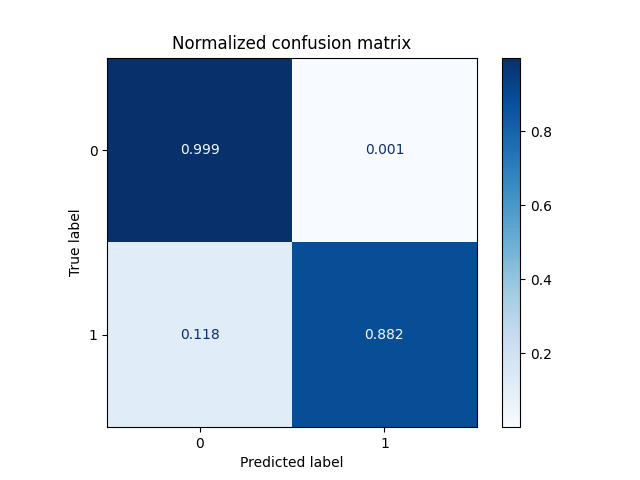
\includegraphics[width=0.75\textwidth]{final-report/img/wednesday/wednesday-baseline-normalized.png}

    \centering
    \begin{tabular}{ |c|c|c|c|c|c|c| }
     \hline
      & true non-attack & true attack \\
     \hline
     predicted non-attack & 1649 & 1 \\
     \hline
     predicted attack & 2 & 15 \\
     \hline
    \end{tabular}
    \caption{Confusion matrices with normalized and absolute values of the baseline model for the experiment 2}
    \label{fig-exp2-baseline}
\end{figure}


\clearpage

\subsubsection{Tuesday}
In this experiment we work with CIC-IDS 2017 Tuesday data set. We sampled $5\ 500$ non-attacks and we kept all 11 attacks. Splitting the data set into train and test sets results in $3\ 850$ non-attacks and 37 attacks in the train set and 1650 non attacks and 4 attacks in the test set.

The confusion matrices for the obtained model in Figure \ref{fig-exp4-transcriptions} again show promising results.

By comparing the baseline model results in the Figure \ref{fig-exp3-baseline} to the results of the obtained model, we conclude that the both models performed the same well.


\begin{figure}[h!]
    \centering
    \includegraphics[width=0.75\textwidth]{final-report/img/tuesday/confusion-matrix-normalized.png}

    \centering
    \begin{tabular}{ |c|c|c|c|c|c|c| }
     \hline
      & true non-attack & true attack \\
     \hline
     predicted non-attack & 1650 & 0 \\
     \hline
     predicted attack & 1 & 3 \\
     \hline
    \end{tabular}
    \caption{Confusion matrix with absolute values for the experiment 3}
    \label{fig-exp3-transcriptions}
\end{figure}


\begin{figure}[h!]
    \centering
    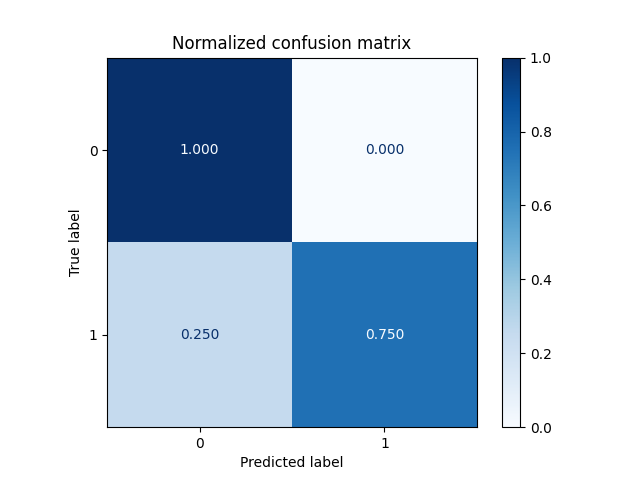
\includegraphics[width=0.75\textwidth]{final-report/img/tuesday/tuesday-baseline-normalized.png}

    \centering
    \begin{tabular}{ |c|c|c|c|c|c|c| }
     \hline
      & true non-attack & true attack \\
     \hline
     predicted non-attack & 1650 & 0 \\
     \hline
     predicted attack & 1 & 3 \\
     \hline
    \end{tabular}
    \caption{Confusion matrices with normalized and absolute values of the baseline model for the experiment 3}
    \label{fig-exp3-baseline}
\end{figure}

\clearpage


\subsubsection{Thursday}
In this experiment we work with CIC-IDS 2017 Thursday data set.

The data set contains $77\ 069$ entries out of which only $1\ 121$ are attacks. We sampled $20\ 000$ non-attacks and we kept all $1\ 121$ attacks. Splitting the data set into train and test sets results in $14\ 000$ non-attacks and 784 attacks in the train set and $6\ 000$ non attacks and 337 attacks in the test set.

The confusion matrices in Figure \ref{fig-exp4-transcriptions} show worse results than in the previous experiments with attacks classification precision nearly $40\%$ and non-attacks classification precision $77.6\%$.

The baseline model scores better results than the obtained model here. We can observe its results in the Figure \ref{fig-exp4-baseline}. The precision of non-attacks classification is about $10\%$ higher than in the obtained model and the precision of attacks classification is about $16\%$ higher than in the obtained model.


\begin{figure}[h!]
    \centering
    \includegraphics[width=0.75\textwidth]{final-report/img/thursday/confusion-matrix-normalized.png}

    \centering
    \begin{tabular}{ |c|c|c|c|c|c|c| }
     \hline
      & true non-attack & true attack \\
     \hline
     predicted non-attack & 4655 & 1345 \\
     \hline
     predicted attack & 203 & 134 \\
     \hline
    \end{tabular}
    \caption{Confusion matrix with absolute values for the experiment 4}
    \label{fig-exp4-transcriptions}
\end{figure}


\begin{figure}[h!]
    \centering
    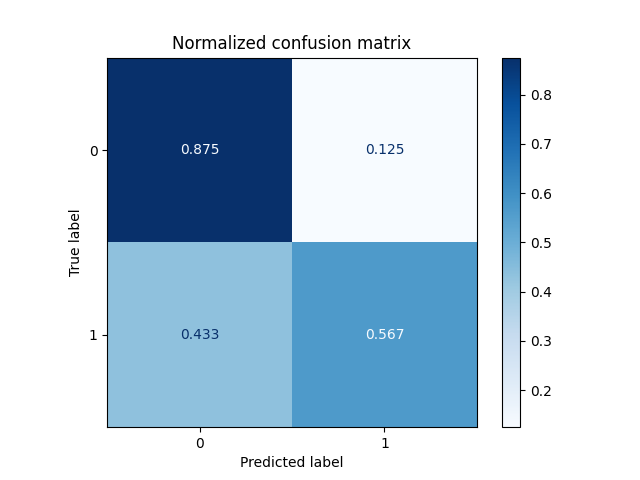
\includegraphics[width=0.75\textwidth]{final-report/img/thursday/baseline-normalized.png}

    \centering
    \begin{tabular}{ |c|c|c|c|c|c|c| }
     \hline
      & true non-attack & true attack \\
     \hline
     predicted non-attack & 5252 & 748 \\
     \hline
     predicted attack & 146 & 191 \\
     \hline
    \end{tabular}
    \caption{Confusion matrices with normalized and absolute values of the baseline model for the experiment 4}
    \label{fig-exp4-baseline}
\end{figure}




\clearpage
\section{Conclusions}
In all experiments baseline models scored better results than the obtained models except of one experiment where they both achieved the very same results. However, in most cases the baseline models performed just slightly better than the obtained models. This means that the very first outcomes in regards to the transcriptions data set look promising.

One potential reason why our obtained models did not succeed in scoring better results than the baseline models is lack of train data. The transformation of transcription data sets into bag of words data set was failing on bigger data sets due to insufficient RAM. This is the reason why we subsampled only certain amount of non-attack samples for each experiment. Using more samples to be transformed into bag of words was crashing our scripts.

Next potential improvement may be choosing a different model instead of Random Forest on top of bag of words and evaluating its results. Using a simple bag of words may be too naive method. Researching and using a different kind of technique may score better results.

Giving more attention to train and test set splits is another kind of improvement. As mentioned in the section \ref{sec-cic-ids-experiments}, the obtained and the baseline models are not necessarily trained and tested on the same network flows. On such few data points a slight shuffle in train and test data may play a big role in the final results. Therefore conducting experiments that train both an obtained model and a baseline model in each experiment on the very same network flows and evaluate their performance on the same test sets may give us more higher quality results.

Regarding the implementation of transcription maker software itself, one may try experimenting with IP packet lengths binning. Would be worth reconsidering the binning approach and assigning more characters to express the packets of lengths $<= 5\ 000$ in order to better express variability among these.


\clearpage
\bibliographystyle{plain}
\bibliography{references}


% \bibliographystyle{plain}

% \begin{thebibliography}{}

% \bibitem{cic-ids-dataset} Iman Sharafaldin, Arash Habibi Lashkari, and Ali A. Ghorbani, “Toward Generating a New Intrusion Detection Dataset and Intrusion Traffic Characterization”, 4th International Conference on Information Systems Security and Privacy (ICISSP), Portugal, January 2018


% % \bibitem{tshark-documentation} Wireshark.org. 2020. \textit{Tshark - The Wireshark Network Analyzer 3.4.0}. [online] Available at: \url{https://www.wireshark.org/docs/man-pages/tshark.html} [Accessed 28 November 2020].

% % \bibitem{python-popularity} Piatetsky, G., 2020. \textit{Python Leads The 11 Top Data Science, Machine Learning Platforms: Trends And Analysis - Kdnuggets}. [online] KDnuggets. Available at: \url{https://www.kdnuggets.com/2019/05/poll-top-data-science-machine-learning-platforms.html} [Accessed 28 November 2020].


% \end{thebibliography}

\end{document}
